\section*{Outline}
\begin{frame}{Notions of Security for Encryption Schemes}
\begin{figure}
\includegraphics[width=.85\textwidth]{ss.png}
\end{figure}
\begin{itemize}
\item<+-> Basic notion of security--\alert{semantic security} \inlinecite{GM'82}.
\begin{itemize}
\item<.-> Security game paramterized by bit $b$ (unknown to adversary)
\item<.-> Adversary is given public parameters (if any)
\item<.-> Can send challenger two messages $m_0$ and $m_1$ of \onslide*<1-2>{her choice}\onslide*<3->{\alert{\textbf{her choice}}}
\item<.-> Receives encryption of message $m_b$
\end{itemize}
\item<+-> For security, adversary must be able guess $b$ with probability at most negligibly greater than $1/2$.
\item<+-> Adversary cannot receive encryptions of key-dependent messages. 
\item<+-> Can plaintexts ever be key-dependent? 
\end{itemize}
\end{frame}
\begin{frame}{Circular and Key-Dependent Message Security}
  \begin{figure}
    \jnote{FIX: Label either via LaTex or picture Alice, Bob, put Eve
      in there somewhere and make a biblical funny, i.e.  ciphertext
      is the fruit}
    \includegraphics[width=.25\textwidth]{circularsecuresnake2.png}
  \end{figure}
  \begin{block}{Can Plaintext Be Key-Dependent?}
    \begin{itemize}
    \item<+-> Yes!
      \begin{itemize}
      \item<.-> Careless or Improper key management
      \item<.-> Integral part of cryptosystem: Gentry's
        ``bootstrapping'' for FHE requires circular-security of secret
        key \inlinecite{Gentry'09}
      \end{itemize}
    \item<+-> Previous results in KDM-security focused on \alert{symmetric}
      and \alert{public-key} encryption and applications, e.g
      \inlinecite{BHHO'08 (DDH), HH'09, ACPS'09 (LWE),BG'10 (QR),
        App'11, MTY'11, BGK'11,BV'11}
    \end{itemize}
  \end{block}

\end{frame}

  \begin{frame}{KDM Attack Model}
    \begin{enumerate}
    \item<1-> Challenger parameterized by bit $b$:\\ sends adversary
      public keys of $d$ arbitrary users
    \item<2-> Adversary makes key-dependent message queries
      \begin{itemize}
      \item<3-> Note: Single-message and multiple-message models
        \alert{NOT} equivalent
      \end{itemize}
    \item<4-> Adversary eventually outputs guess $b'$
    \end{enumerate}
    \begin{figure}
      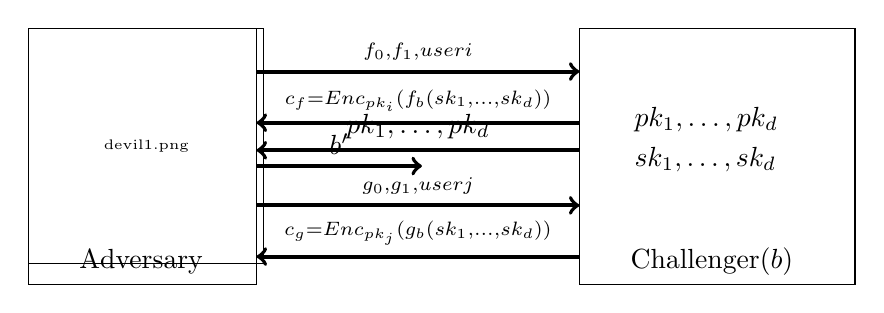
\begin{tikzpicture}
     
     	% Adversary picture/text
        \pgfdeclareimage[interpolate=true,width=3cm,height=3cm]{adversary}{devil1.png}
        \pgftext[at=\pgfpoint{0cm}{-0.25cm},left,base]{\pgfuseimage{adversary}}
        \pgftext[at=\pgfpoint{.65cm}{-0.3cm},left,base]{Adversary}
        \pgfpathrectangle{\pgfpoint{0.0cm}{-0.5cm}}{\pgfpoint{2.9cm}{3.25cm}}

        % \pgftext[at=\pgfpoint{1.2cm}{0.05cm},left,base]{A}
        
        % Challenger picture/text 
                \pgfpathrectangle{\pgfpoint{7cm}{-0.5cm}}{\pgfpoint{3.5cm}{3.25cm}} % Box
        \pgftext[at=\pgfpoint{7.65cm}{-0.3cm},left,base]{Challenger($b$)}
        \pgftext[at=\pgfpoint{7.7cm}{1.5cm},left,base]{$
          pk_1, \ldots, pk_d$}
         \pgftext[at=\pgfpoint{7.7cm}{1.0cm},left,base]{$sk_1, \ldots, sk_d$}




    %    \pgfpathrectangle{\pgfpoint{6.75cm}{1cm}}{\pgfpoint{3cm}{1cm}} % Encryption box
       	% public keys sent to adversary
        \pgfusepath{stroke} 
        
        
        \onslide<1|handout:0>{ \draw[->,line
          width=0.05cm] (7.00cm, 1.2cm) -- (2.9cm, 1.2cm)
          node[midway,above] {$pk_1, \ldots, pk_d$}; }
          
         % Sends first function 
        \onslide<2-3|handout:1>{ \draw[->, line width=0.05cm] (2.9cm,
          2.2cm) -- (7.00cm, 2.2cm) node[midway, above]{$\scriptstyle f_0, f_1,
            \text{user } i$};

       
          \draw[->, line width=0.05cm] (7.00cm,1.55cm) --     (2.9, 1.55cm)
          node[midway, above]{$\scriptstyle
            c_{f}=\text{Enc}_{pk_{i}}(f_{b}( sk_1, \ldots, sk_{d}))$};     
 
        }

        \onslide<3|handout:0>{ \draw[->, line width=0.05cm] (2.9cm,
          0.5cm) -- (7.00cm, 0.5cm) node[midway, above]{$\scriptstyle g_0, g_1,
            \text{user } j$};

          \draw[->, line width=0.05cm] (7.00cm,-0.15cm) -- (2.9cm,
          -0.15cm) node[midway, above]{$\scriptstyle
            c_{g}=\text{Enc}_{pk_{j}}(g_{b}( sk_1, \ldots, sk_{d}))$};


        }

        \onslide<4-|handout:0>{ \draw[->,line width=0.05cm] (2.9cm,
          1cm) -- (5cm, 1cm) node[midway, above]{$b'$}; }

      \end{tikzpicture}
    \end{figure}

  \end{frame}

\begin{frame}{Identity-Based Encryption}
\begin{itemize}
\item<+-> Normal public-key encryption
\begin{itemize}
\item<.-> Public keys unrelated to a
  user's identity
\smallskip
\item<.-> Requires cumbersome public key infrastructure, certificates
\end{itemize}
\item<+-> Identity-based encryption
\begin{itemize}
\item<.-> Public keys are user's identities,
  i.e. \textsf{jmas6@cc.gatech.edu}
\smallskip
\item<.-> Private key generator with master secret key generates user
  secret keys
\end{itemize}
\item<+-> Security for Identity-Based Encryption
\begin{itemize}
\item<.-> Adversary may request secret keys for identities of her
  choice
\smallskip
\item<+-> \alert{Selective Security}-Adversary must specify identity
  to attack before seeing any public parameters of scheme
\smallskip
\item<+-> \alert{Adaptive Security}-Adversary may request secret keys
before specifying the challenge identity
\end{itemize}
\end{itemize}
\end{frame}



\begin{frame}{KDM Security for Identity-Based Encryption}
Key-dependent messages arise naturally in identity-based encryption
  \begin{itemize}
  \item<+-> IBE for revocation: user identity at epoch
    $i$ is $\text{id} := \text{username}||i$\\
 PKG sends key for next epoch by encrypting it under
    previous identity.
  \item<+-> What if user deleted old key, wants to decrypt old
    ciphertext?
  \item<+-> Solution: PKG sends old key encrypted under
    current epoch's identity.
  \item<+-> May be unsafe if the IBE is not KDM-secure
  \end{itemize}
  \begin{overprint}
  \begin{figure}
    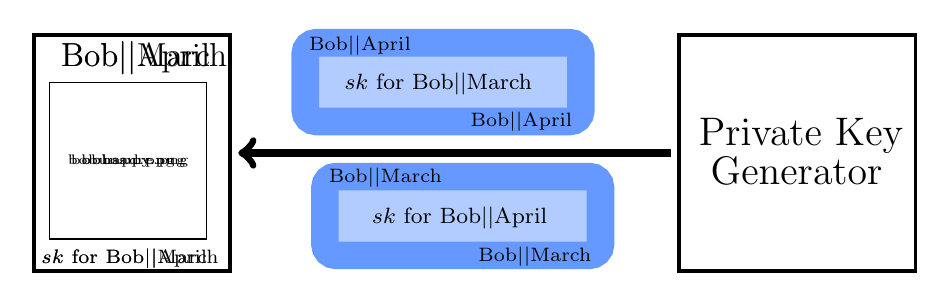
\begin{tikzpicture}
      \definecolor{superlightblue}{rgb}{0.7,0.8,1}
      \definecolor{lightblue}{rgb}{0.4,0.6,1}
      \pgfdeclareimage[interpolate=true,width=2cm,height=2cm]{bobhappy}{bobhappy.png}
      \pgfdeclareimage[interpolate=true,width=2cm,height=2cm]{bobsad}{bobsad.png}
      \pgfdeclareimage[interpolate=true,width=2cm,height=2cm]{bobunsure}{bobunsure.png}
      \draw [draw=black, line width=.05cm] (8cm,0cm)
      rectangle (11cm, 3cm); 
      
      \draw [draw=black, line width=.05cm] (-0.2cm,0cm) rectangle (2.3cm, 3cm);
      \onslide*<1,3|handout:0>{\pgftext[at=\pgfpoint{0cm}{0.4cm},left,base]{\pgfuseimage{bobhappy}}
      }
      \onslide*<2|handout:0>{\pgftext[at=\pgfpoint{0cm}{0.4cm},left,base]{\pgfuseimage{bobunsure}}
      }
      \onslide*<4|handout:1>{\pgftext[at=\pgfpoint{0cm}{0.4cm},left,base]{\pgfuseimage{bobsad}}
      }


      \pgftext[at=\pgfpoint{8.25cm}{1.6cm},left,base]{\Large Private
        Key} \pgftext[at=\pgfpoint{8.4cm}{1.1cm},left,base]{\Large
        Generator}

      \draw[<-, line width=.1cm,black] (2.4cm, 1.5cm) -- (7.9cm,
      1.5cm);

      \onslide<1|handout:0>{\pgftext[at=\pgfpoint{0.15cm}{2.6cm},left,base]{\large
          Bob$||$March}

        \pgftext[at=\pgfpoint{-0.1cm}{0.1cm},left,base]{\scriptsize
          $sk$ for Bob$||$March} }


      \onslide<2-4|handout:1>{\pgftext[at=\pgfpoint{0.15cm}{2.6cm},left,base]{\large
          Bob$||$April}

        \pgftext[at=\pgfpoint{-0.1cm}{0.1cm},left,base]{\scriptsize
          $sk$ for Bob$||$April} } 
          
          \onslide<1-4>{ \filldraw
        [draw=lightblue, line width=.35cm, rounded corners,
        fill=superlightblue] (3.5cm,0.2cm) rectangle (7cm,1.2cm);

	\pgftext[at=\pgfpoint{5.45cm}{0.12cm},left,base]{\scriptsize
          Bob$||$March}
	
	\pgftext[at=\pgfpoint{3.55cm}{1.12cm},left,base]{\scriptsize
          Bob$||$March} } 


      \onslide<1-4|handout:1>{\pgftext[at=\pgfpoint{4.1cm}{0.6cm},left,base]{\footnotesize
          $sk$ for Bob$||$April}}



      \onslide<3-4|handout:1>{ \filldraw [draw=lightblue, line width=.35cm,
        rounded corners, fill=superlightblue] (3.25cm,1.9cm) rectangle
        (6.75cm,2.9cm);
        \pgftext[at=\pgfpoint{3.75cm}{2.3cm},left,base]{\footnotesize
          $sk$ for Bob$||$March}
        \pgftext[at=\pgfpoint{5.35cm}{1.83cm},left,base]{\scriptsize
          Bob$||$April}
	
	\pgftext[at=\pgfpoint{3.3cm}{2.8cm},left,base]{\scriptsize
          Bob$||$April} }
    \end{tikzpicture}
%\includegraphics<2|handout:0>[width=.8\textwidth]{realnewkey.png}
%\includegraphics<3|handout:1>[width=.8\textwidth]{realoldkey.png}
%\includegraphics<4|handout:0>[width=.8\textwidth]{realoldkeysad.png}
 \end{figure}

\end{overprint}
\end{frame}
%%% Local Variables: 
%%% mode: latex
%%% TeX-master: "slides"
%%% End: 
